\documentclass[10pt]{exam}
\usepackage[phy]{template-for-exam}
\usepackage{graphicx}
\usepackage{enumitem}
\setlist{topsep=0pt,itemsep=-1ex,partopsep=1ex,parsep=1ex}
\usepackage{pgfplots}
\pgfplotsset{
  compat=1.18,
  ylabel={period (s)},
  width=13.5cm,
  height=5.6cm,
  ymin=0,
  ymax=2.5,
  axis y line = left,
  axis x line = bottom,
  grid=both,
  minor tick num = 4,
  axis line style = ultra thick,
  major grid style = black,
  ytick={0,1,...,3},
}

\title{Spring Lab}
\author{Rohrbach}
\date{\today}

\begin{document}
\maketitle


\section*{Purpose} 
  Write one sentence explaining what you are trying to figure out in this lab. Make sure your purpose includes all of your independent and dependent variables

  \vs

\section*{Hypotheses} 
  Predict what the relationship will be between each of your independent variables and your dependent variable (\emph{i.e. directly proportional, inversely proportional, unrelated).} Make sure to explain why you think each of these relationships will hold.

  \emph{Example:} mass and period will be (choose one: directly proportional, inversely proportional, unrelated).
  \vspace{1em}

  Hypothesis \#1:\vspace{1em}

  Explanation \#1: \vspace{3em}

  Hypothesis \#2:\vspace{1em}

  Explanation \#2: \vspace{3em}

  Hypothesis \#3:\vspace{1em}

  Explanation \#3: \vspace{3em}



\section*{Procedure} 
  Make a brief list of the steps you follow in the lab.

  \begin{itemize}
    \item
      Make a list of all three experiments that you will perform.
    \item
      Explain how, specifically, you will be measuring the dependent variable.
    \item
      Explain how many values of each independent variable there will be.

  \end{itemize}

  \vs[3]

  \pagebreak

  \vspace*{\stretch{1}}

\section*{Data}
  Show all data tables for each of your experiments.

  \begin{itemize}
    \item
      Be sure that each data table lists the variables you are holding constant and their values
    \item
      Make sure all units are labeled. (It is OK to label the units in the table headings instead of in each individual cell)
  \end{itemize}

  \vspace{1em}

  \paragraph{Hints:} \hfill

  \begin{enumerate}
    \item 
      When testing \emph{spring constant}, use 150 grams at an amplitude of 5 cm
    \item 
      When testing \emph{amplitude} use one of the narrow springs (7.5~N/m or 2.5~N/m).   Pick a mass that gets an appropriate amount of extension out of the spring without going overboard.
    \item 
      When testing \emph{mass}, make sure to think ahead about which spring and weights to use so that you don't over-stretch the spring.
    
  \end{enumerate}

  \vspace{4em}


  \newcommand{\datatable}[3]{
    \begin{tabular}{|p{8em}|||c|c|c||c|||p{8em}|}
      \hline
      \multicolumn{6}{|l|}{\bf Experiment\##1: #2} \\\hline
      \multicolumn{6}{|l|}{\bf Constant Variables:} \\[.5em] \hline
      &\multicolumn{4}{l|||}{} & \\[.5em] \cline{2-5} 
      & Trial \#1 & Trial \#2 & Trial \#3 & Average & \\ \hline
      &&&&&\\[.5em] \hline
      &&&&&\\[.5em] \hline
      &&&&&\\[.5em] \hline
      &&&&&\\[.5em] \hline
      &&&&&\\[.5em] \hline

    \end{tabular}

    \vspace{2em}

    
  }


  \datatable{1}{Spring Constant vs. Period}

  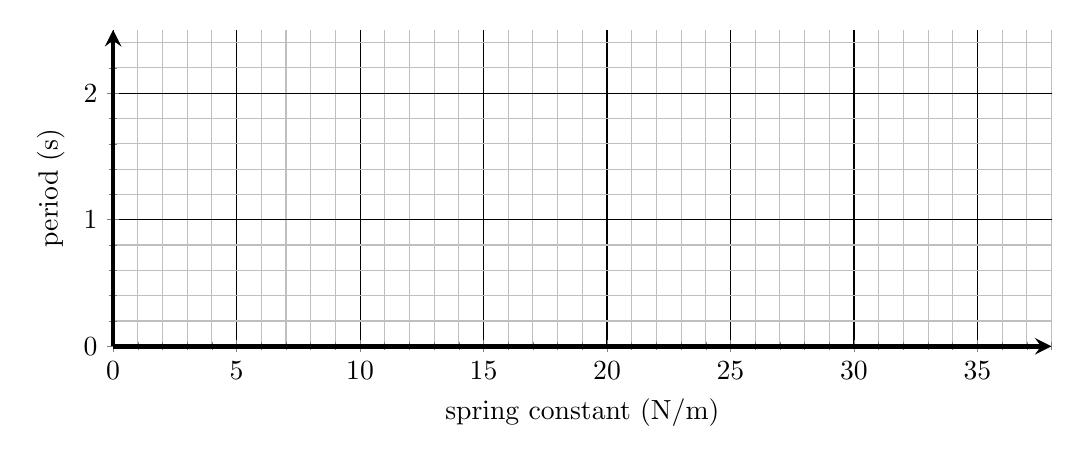
\begin{tikzpicture}
    \begin{axis}[
      xlabel={spring constant (N/m)},
      xtick={0,5,10,...,50},
      xmin=0,
      xmax=38,
    ]
    \end{axis}
  \end{tikzpicture}

  \pagebreak

  \datatable{2}{Amplitude vs. Period}

  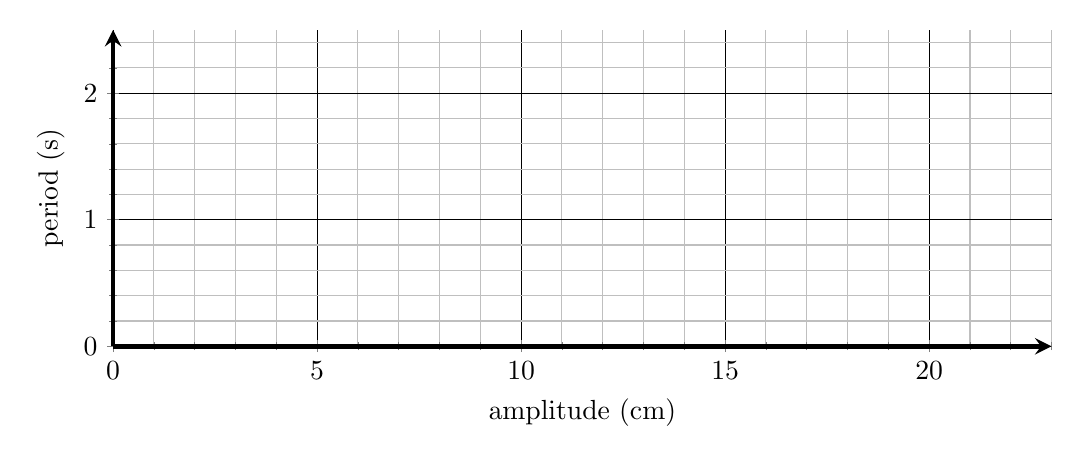
\begin{tikzpicture}
    \begin{axis}[
      xlabel={amplitude (cm)},
      xtick={0,5,...,45},
      xmin=0,
      xmax=23,
    ]
    \end{axis}
  \end{tikzpicture}

  \vs

  \datatable{3}{Mass vs. Period}

    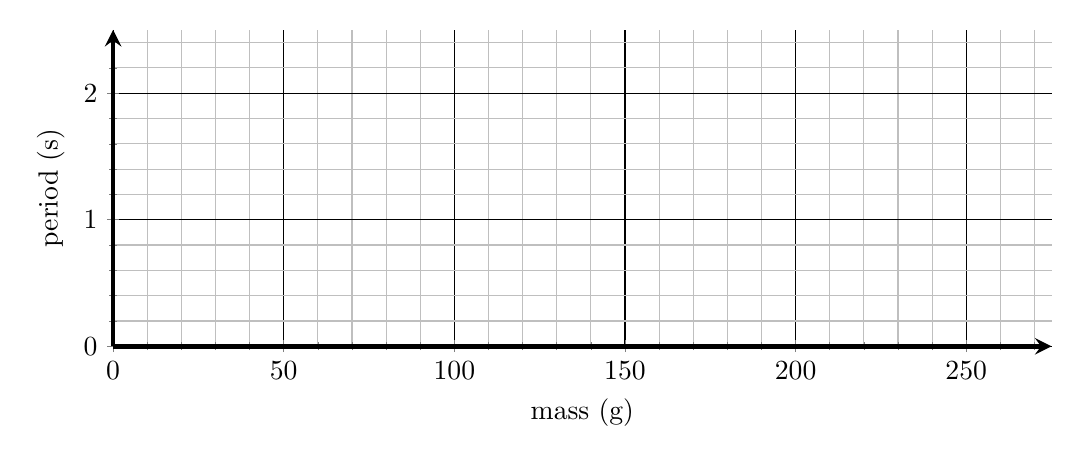
\begin{tikzpicture}
      \begin{axis}[
        xlabel={mass (g)},
        xtick={0,50,...,300},
        xmin=0,
        xmax=275,
      ]
      \end{axis}
    \end{tikzpicture}



\section*{Results} 
  All you need are three sentences for this section: one for each experiment.  Your results should describe the relationship between each of your independent variables and your dependent variable (\emph{i.e. directly proportional, inversely proportional, unrelated)}.
    
  \emph{Example:} Mass and period were unrelated.

  \vspace{3em}

  Result \#1: \vspace{3em} 

  Result \#2: \vspace{3em} 

  Result \#3: \vspace{3em} 




\section*{Conclusion and Discussion}
  Answer the following questions in paragraph form.

  \begin{itemize}
    \item
      What was the purpose of the lab?
    \item
      How did you go about accomplishing the purpose?
    \item
      What did you find (\emph{i.e.} what affected the period of the
      pendulum and how did it affect it)?
    \item
      What errors came up in this lab and how could you correct them in the
      future?
  \end{itemize}

\end{document}